\documentclass[12pt]{article}

\usepackage{fullpage}
\usepackage[round]{natbib}
\usepackage{multirow}
\usepackage{booktabs}
\usepackage{graphicx}
\usepackage{hyperref}

\hypersetup{
    bookmarks=true,         % show bookmarks bar?
    colorlinks=true,       % false: boxed links; true: colored links
    linkcolor=red,          % color of internal links (change box color with linkbordercolor)
    citecolor=green,        % color of links to bibliography
    filecolor=magenta,      % color of file links
    urlcolor=cyan           % color of external links
}
\newcounter{acnum}
\newcommand{\actheacnum}{AC\theacnum}
\newcommand{\acref}[1]{AC\ref{#1}}

\newcounter{ucnum}
\newcommand{\uctheucnum}{UC\theucnum}
\newcommand{\uref}[1]{UC\ref{#1}}

\newcounter{mnum}
\newcommand{\mthemnum}{M\themnum}
\newcommand{\mref}[1]{M\ref{#1}}

%% Comments
\newif\ifcomments\commentstrue

\ifcomments
\newcommand{\authornote}[3]{\textcolor{#1}{[#3 ---#2]}}
\newcommand{\todo}[1]{\textcolor{red}{[TODO: #1]}}
\else
\newcommand{\authornote}[3]{}
\newcommand{\todo}[1]{}
\fi

\newcommand{\wss}[1]{\authornote{magenta}{SS}{#1}}

\begin{document}

\title{Module Guide for Chipmunk2D Game Physics Library} 
\author{Alex Halliwushka and Luthfi Mawarid}
\date{\today}
	
\maketitle

\tableofcontents

\section{Introduction}

Decomposing a system into modules is a commonly accepted approach to developing software.  A module is a work assignment for a programmer or programming team~\citep{ParnasEtAl1984}.  In the best practices for scientific computing, \citet{WilsonEtAl2013} advise a modular design, but are silent on the criteria to use to decompose the software into modules.  We advocate a decomposition based on the principle of information hiding~\citep{Parnas1972a}. This principle supports design for change, because the ``secrets'' that each module hides represent likely future changes.  Design for change is valuable in SC, where modifications are frequent, especially during initial development as the solution space is explored.  \\
\newline
Our design follows the rules laid out by \citet{ParnasEtAl1984}, as follows:
\begin{itemize}
\item System details that are likely to change independently should be the
  secrets of separate modules.
\item Each data structure is used in only one module.
\item Any other program that requires information stored in a module's data
  structures must obtain it by calling access programs belonging to that module.
\end{itemize}

\noindent After completing the first stage of the design, the Software Requirements
Specification (SRS), the Module Guide (MG) is developed~\citep{ParnasEtAl1984}. The MG
specifies the modular structure of the system and is intended to allow both
designers and maintainers to easily identify the parts of the software.  The
potential readers of this document are as follows:

\begin{itemize}
\item New project members: This document can be a guide for a new project member
  to easily understand the overall structure and quickly find the
  relevant modules they are searching for.
\item Maintainers: The hierarchical structure of the module guide improves the
  maintainers' understanding when they need to make changes to the system. It is
  important for a maintainer to update the relevant sections of the document
  after changes have been made.
\item Designers: Once the module guide has been written, it can be used to
  check for consistency, feasibility and flexibility. Designers can verify the
  system in various ways, such as consistency among modules, feasibility of the
  decomposition, and flexibility of the design.
\end{itemize}

\noindent The rest of the document is organized as follows. Section
\ref{SecChange} lists the anticipated and unlikely changes of the software
requirements. Section \ref{SecMH} summarizes the module decomposition that
was constructed according to the likely changes. Section \ref{SecConnection}
specifies the connections between the software requirements and the
modules. Section \ref{SecMD} gives a detailed description of the
modules. Section \ref{SecTM} includes two traceability matrices. One checks
the completeness of the design against the requirements provided in the SRS. The
other shows the relation between anticipated changes and the modules. Section
\ref{SecUse} describes the use relation between modules.

\section{Anticipated and Unlikely Changes} \label{SecChange}

This section lists possible changes to the system. According to the likeliness
of the change, the possible changes are classified into two
categories. Anticipated changes are listed in Section \ref{SecAchange}, and
unlikely changes are listed in Section \ref{SecUchange}.

\subsection{Anticipated Changes} \label{SecAchange}

Anticipated changes are the source of the information that is to be hidden
inside the modules. Ideally, changing one of the anticipated changes will only
require changing the one module that hides the associated decision. The approach
adapted here is called design for
change. %Anticipated changes are numbered by \textbf{AC} followed by a number.

\begin{description}
\item[\refstepcounter{acnum} \actheacnum \label{acHardware}:] The specific
  hardware on which the software is running.
\item[\refstepcounter{acnum} \actheacnum \label{acBody}:] The data structure of the
physical properties of an object such as the object's mass, position and velocity.
\item[\refstepcounter{acnum} \actheacnum \label{acShape}:] The data structure of the
surface properties of an object such as the object's friction and elasticity.
\item[\refstepcounter{acnum} \actheacnum \label{acSpace}:] How all the rigid
bodies and shapes interact together.
\item[\refstepcounter{acnum} \actheacnum \label{acCollision}:] The data structure containing collision information such as the objects that collide and their mass. 
\item[\refstepcounter{acnum} \actheacnum \label{acControl}:] How the overall
  control of the simulation is orchestrated, including the input and output of data.
\item[\refstepcounter{acnum} \actheacnum \label{acVector}:] The implementation of mathematical vectors.
\item[\refstepcounter{acnum} \actheacnum \label{acBBox}:] The implementation of bounding box structures.
\item[\refstepcounter{acnum} \actheacnum \label{acTrans}:] The implementation of transformation matrices.
\item[\refstepcounter{acnum} \actheacnum \label{acSpatialIndex}:] How the simulation space is spatially indexed.
\item[\refstepcounter{acnum} \actheacnum \label{acSolver}:] The algorithm used for solving collisions.
\item[\refstepcounter{acnum} \actheacnum \label{acSeqDS}:] The implementation
  for the sequence (array) data structure.
\item[\refstepcounter{acnum} \actheacnum \label{acLinkDS}:] The implementation for the linked (tree) data structure.
\item[\refstepcounter{acnum} \actheacnum \label{acAssocDS}:] The implementation
  for the associative (hash table) data structure.
\end{description}

\subsection{Unlikely Changes} \label{SecUchange}

The module design should be as general as possible. However, a general system is
more complex. Sometimes this complexity is not necessary. Fixing some design
decisions at the system architecture stage can simplify the software design. If
these decision should later need to be changed, then many parts of the design
will potentially need to be modified. Hence, it is not intended that these
decisions will be changed. 

\begin{description}
\item[\refstepcounter{ucnum} \uctheucnum \label{ucIO}:] Input/Output devices
  (Input: Keyboard and/or mouse, Output: Memory and/or Screen).
\item[\refstepcounter{ucnum} \uctheucnum \label{ucInput}:] There will always be a source of input data external to the software.
\item[\refstepcounter{ucnum} \uctheucnum \label{ucOutput}:] Output data are
  displayed to the output device.
\item[\refstepcounter{ucnum} \uctheucnum \label{ucGoal}:] The goal of the system is to simulate the interactions of 2D rigid bodies.
\item[\refstepcounter{ucnum} \uctheucnum \label{ucCartesian}:] A Cartesian 
coordinate system is used.
\item[\refstepcounter{ucnum} \uctheucnum \label{ucRigid}:] All objects
are rigid bodies.
\item[\refstepcounter{ucnum} \uctheucnum \label{uc2D}:] All objects
are 2D.
\end{description}

\section{Module Hierarchy} \label{SecMH}

This section provides an overview of the module design. Modules are summarized
in a hierarchy decomposed by secrets in Table \ref{TblMH}. The modules listed
below, which are leaves in the hierarchy tree, are the modules that will
actually be implemented.

\begin{description}
\item [\refstepcounter{mnum} \mthemnum \label{mHH}:] Hardware-Hiding Module 
\item [\refstepcounter{mnum} \mthemnum \label{mBody}:] Rigid Body Module 
\item [\refstepcounter{mnum} \mthemnum \label{mShape}:] Shape Module 
\item [\refstepcounter{mnum} \mthemnum \label{mCircle}:] Circle Module
\item [\refstepcounter{mnum} \mthemnum \label{mSegment}:] Segment Module
\item [\refstepcounter{mnum} \mthemnum \label{mPoly}:] Polygon Module
\item [\refstepcounter{mnum} \mthemnum \label{mSpace}:] Space Module 
\item [\refstepcounter{mnum} \mthemnum \label{mCollision}:] Arbiter Module 
\item [\refstepcounter{mnum} \mthemnum \label{mControl}:] Control Module 
\item [\refstepcounter{mnum} \mthemnum \label{mVector}:] Vector Module
\item [\refstepcounter{mnum} \mthemnum \label{mBBox}:] Bounding Box Module
\item [\refstepcounter{mnum} \mthemnum \label{mTrans}:] Transform Matrix Module
\item [\refstepcounter{mnum} \mthemnum \label{mSpatialIndex}:] Spatial Index Module
\item [\refstepcounter{mnum} \mthemnum \label{mSolver}:] Collision Solver Module 
\item [\refstepcounter{mnum} \mthemnum \label{mSeqDS}:] Sequence Data Structure Module
\item [\refstepcounter{mnum} \mthemnum \label{mLinkDS}:] Linked Data Structure Module  
\item [\refstepcounter{mnum} \mthemnum \label{mAssocDS}:] Associative Data Structure Module 
\end{description}
\noindent
Note that \mref{mHH} is a commonly used module and is already implemented by the operating
system.  It will not be reimplemented.

\begin{table}[h!]
\centering
\begin{tabular}{p{0.3\textwidth} p{0.4\textwidth} p{0.3\textwidth}}
\toprule
\textbf{Level 1} & \textbf{Level 2}  & \textbf{Level 3} \\
\midrule

{Hardware-Hiding Module} & ~ \\
\midrule

\multirow{7}{0.3\textwidth}{Behaviour-Hiding Module} 
& Rigid Body Module \\
& \multirow{3}{0.3\textwidth}{Shape Module} 
& Circle Module \\
& &Segment Module \\
& &Polygon Module \\
& Space Module \\ 
& Arbiter Module \\
& Control Module \\
\midrule
\multirow{8}{0.3\textwidth}{Software Decision Module} 
& Vector Module \\
& Transform Matrix Module \\
& Bounding Box Module \\
& Spatial Index Module \\
& Collision Solver Module \\  
& Sequence Data Structure Module \\  
& Linked Data Structure Module \\  
& Associative Data Structure Module \\  
\bottomrule

\end{tabular}
\caption{Module Hierarchy}
\label{TblMH}
\end{table}

\section{Connection Between Requirements and Design} \label{SecConnection}

The design of the system is intended to satisfy the requirements developed in
the SRS. In this stage, the system is decomposed into modules. The connection
between requirements and modules is listed in Table \ref{TblRT}.

\section{Module Decomposition} \label{SecMD}

Modules are decomposed according to the principle of ``information hiding''
proposed by \citet{ParnasEtAl1984}. The \emph{Secrets} field in a module
decomposition is a brief statement of the design decision hidden by the
module. The \emph{Services} field specifies \emph{what} the module will do
without documenting \emph{how} to do it. For each module, a suggestion for the implementing software is given under the \emph{Implemented By} title. If the entry is \emph{OS}, this means that the module is provided by the operating system or by standard programming language libraries. If the entry is \emph{Chipmunk}, this means that the module will be implemented by the 
game physics library.  
% should reference a command for the name, in case it changes
If a dash (\emph{--}) is shown, this means
that the module is not a leaf and will not have to be implemented. Whether or
not this module is implemented depends on the programming language
selected.
If a module has a children section, the modules listed will inherit from  
this module. Both the parent and the children modules will be implemented.

\subsection{Hardware Hiding Modules (\mref{mHH})}

\begin{description}
\item[Secrets:]The data structure and algorithm used to implement the virtual
  hardware.
\item[Services:] Serves as a virtual hardware used by the rest of the
  system. This module provides the interface between the hardware and the
  software. So, the system can use it to display outputs or to accept inputs.
\item[Implemented By:] OS
\end{description}

\subsection{Behaviour-Hiding Module}

\begin{description}
\item[Secrets:]The contents of the required behaviours.
\item[Services:]Includes programs that provide externally visible behavior of
  the system as specified in the software requirements specification (SRS)
  documents. This module serves as a communication layer between the
  hardware-hiding module and the software decision module. The programs in this module will need to change if there are changes in the SRS.
\item[Implemented By:] --
\end{description}

\subsubsection{Rigid Body Module (\mref{mBody})}

\begin{description}
\item[Secrets:]The data structure of a rigid body.
\item[Services:]Stores the physical properties of an object, such as mass, 
position, rotation, velocity, etc, and provides operations on rigid bodies, such as setting the mass and velocity of the body.

\item[Implemented By:] Chipmunk
\end{description}

\subsubsection{Shape Module (\mref{mShape})}

\begin{description}
\item[Secrets:]The data structure of a collision shape.
\item[Services:]Stores the surface properties of an object, such as friction or elasticity, and provides operations on shapes, such as setting its friction or elasticity.
\item[Children:] Circle Module, Segment Module, Polygon Module
\item[Implemented By:] Chipmunk
\end{description}

\paragraph{Circle Module (\mref{mCircle})}

\begin{description}
	\item[Secrets:] The data structure of a circle shape.
	\item[Services:] Provides operations on circles such as initializing a new circle, calculating moment and area, etc.
	\item[Implemented By:] Chipmunk
\end{description}

\paragraph{Segment Module (\mref{mSegment})}

\begin{description}
	\item[Secrets:] The data structure of a segment shape.
	\item[Services:] Provides operations on segments such as initializing a new segment, calculating moment and area, etc.
	\item[Implemented By:] Chipmunk
\end{description}

\paragraph{Polygon Module (\mref{mPoly})}

\begin{description}
	\item[Secrets:] The data structure of a polygon shape.
	\item[Services:] Provides operations on polygons such as initializing a new polygon, calculating moment, area and centroid, etc.
	\item[Implemented By:] Chipmunk
\end{description}

\subsubsection{Space Module (\mref{mSpace})}

\begin{description}
	\item[Secrets:] The container for simulating objects.
	\item[Services:]Controls how all the rigid bodies and shapes interact together.
	\item[Implemented By:] Chipmunk
\end{description} 

\subsubsection{Arbiter Module (\mref{mCollision})}

\begin{description}
\item[Secrets:]The data structure containing collision information.
\item[Services:]Stores all collision data, such as which bodies 
collided and their masses.
\item[Implemented By:] Chipmunk
\end{description}
 
\subsubsection{Control Module (\mref{mControl})}

\begin{description}
\item[Secrets:] The algorithm for coordinating the running of the program and the interface for receiving inputs and sending outputs.
\item[Services:] Provides the main program.
\item[Implemented By:] Chipmunk
\end{description}

\subsection{Software Decision Module}

\begin{description}
\item[Secrets:] The design decision based on mathematical theorems, physical
  facts, or programming considerations. The secrets of this module are
  \emph{not} described in the SRS.
\item[Services:] Includes data structure and algorithms used in the system that do not provide direct interaction with the user. 
  % Changes in these modules are more likely to be motivated by a desire to
  % improve performance than by externally imposed changes.
\item[Implemented By:] --
\end{description}

\subsubsection{Vector Module (\mref{mVector})}
	
\begin{description}
	\item[Secrets:] The data structure representing vectors.
	\item[Services:] Provides vector operations such as addition, scalar and vector multiplication, dot and cross products, rotations, etc.
	\item[Implemented By:] Chipmunk
\end{description}

\subsubsection{Bounding Box Module (\mref{mBBox})}

\begin{description}
	\item[Secrets:] The data structure for representing bounding boxes.
	\item[Services:] Provides constructors for bounding boxes and operations such as merging boxes, calculating their centroids and areas, etc.
	\item[Implemented By:] Chipmunk
\end{description}

\subsubsection{Transform Matrix Module (\mref{mTrans})}

\begin{description}
	\item[Secrets:] The data structure representing transformation matrices.
	\item[Services:] Provides constructors for affine transformation matrices, matrix operations such as inverse, transpose, multiplications, and operations for applying transformations to vectors and bounding boxes.
	\item[Implemented By:] Chipmunk
\end{description}

\subsubsection{Spatial Index Module (\mref{mSpatialIndex})}

\begin{description}
	\item[Secrets:] The data structures and algorithms for spatially indexing the simulation space.
	\item[Services:] Provides spatial indexing operations and tracks the positions of bodies in the simulation space.
	\item[Implemented By:] Chipmunk
\end{description}

\subsubsection{Collision Solver Module (\mref{mSolver})}

\begin{description}
	\item[Secrets:] The data structures and algorithms for detecting collisions.
	\item[Services:] Fast collision filtering, primitive shape to shape collision detection.
	\item[Implemented By:] Chipmunk
\end{description}

\subsubsection{Sequence Data Structure Module (\mref{mSeqDS})}

\begin{description}
\item[Secrets:] The data structure for a sequence data type.
\item[Services:] Provides array manipulation operations, such as building an array, accessing a specific entry, slicing an array, etc.
\item[Implemented By:] Chipmunk
\end{description}

\subsubsection{Linked Data Structure Module (\mref{mLinkDS})}

\begin{description}
\item[Secrets:] The data structure for a linked data type.
\item[Services:] Provides tree manipulation operations, such as building a tree, accessing a specific entry, etc.
\item[Implemented By:] Chipmunk
\end{description}

\subsubsection{Associative Data Structure Module (\mref{mAssocDS})}

\begin{description}
\item[Secrets:] The data structure for an associative data type.
\item[Services:] Provides operations on hash tables, such as building a hash table, accessing a specific entry, etc.
\item[Implemented By:] Chipmunk
\end{description}

~\newpage

\section{Traceability Matrix} \label{SecTM}

This section shows two traceability matrices: between the modules and the
requirements, and between the modules and the anticipated changes. We should also consider documenting the mapping between these ``abstract" modules and the C files.

% the table should use mref, the requirements should be named, use something
% like fref
\begin{table}[h!]
\centering
\begin{tabular}{p{0.2\textwidth} p{0.6\textwidth}}
\toprule
\textbf{Req.} & \textbf{Modules}\\
\midrule
	R1 & M\ref{mSpace}, M\ref{mControl}, M\ref{mSeqDS} \\
	R2 & M\ref{mBody}, M\ref{mControl}, M\ref{mVector}, M\ref{mTrans} \\
	R3 & M\ref{mShape}, M\ref{mCircle}, M\ref{mSegment}, M\ref{mPoly}, M\ref{mControl}, M\ref{mVector} \\
	R4 & M\ref{mBody}, M\ref{mShape}, M\ref{mCircle}, M\ref{mSegment}, M\ref{mPoly}, M\ref{mSpace}, M\ref{mControl} \\
	R5 & M\ref{mBody}, M\ref{mSpace}, M\ref{mVector}, M\ref{mTrans} \\
	R6 & M\ref{mBody}, M\ref{mSpace}, M\ref{mVector}, M\ref{mTrans} \\
	R7 & M\ref{mBody}, M\ref{mSpace}, M\ref{mBBox}, M\ref{mSpatialIndex}, M\ref{mSolver}, M\ref{mLinkDS}, M\ref{mAssocDS} \\
	R8 & M\ref{mBody}, M\ref{mSpace}, M\ref{mVector}, M\ref{mTrans}, M\ref{mCollision} \\
\bottomrule
\end{tabular}
\caption{Trace Between Requirements and Modules}
\label{TblRT}
\end{table}

\begin{table}[h!]
\centering
\begin{tabular}{p{0.2\textwidth} p{0.6\textwidth}}
\toprule
	\textbf{AC} & \textbf{Modules}\\
\midrule
	AC\ref{acHardware} & M\ref{mHH} \\
	AC\ref{acBody} & M\ref{mBody} \\
	AC\ref{acShape} & M\ref{mShape}, M\ref{mCircle}, M\ref{mSegment}, M\ref{mPoly} \\
	AC\ref{acSpace} & M\ref{mSpace} \\
	AC\ref{acCollision} & M\ref{mCollision} \\
	AC\ref{acControl} & M\ref{mControl} \\
	AC\ref{acVector} & M\ref{mVector} \\
	AC\ref{acBBox} & M\ref{mBBox} \\
	AC\ref{acTrans} & M\ref{mTrans} \\
	AC\ref{acSpatialIndex} & M\ref{mSpatialIndex} \\
	AC\ref{acSolver} & M\ref{mSolver} \\
	AC\ref{acSeqDS} & M\ref{mSeqDS} \\
	AC\ref{acLinkDS} & M\ref{mLinkDS} \\
	AC\ref{acAssocDS} & M\ref{mAssocDS} \\
\bottomrule
\end{tabular}
\caption{Trace Between Anticipated Changes and Modules}
\label{TblAT}
\end{table}

~\newpage

\section{Use Hierarchy Between Modules} \label{SecUse}

In this section, the uses hierarchy between modules is
provided. \citet{Parnas1978} said of two programs A and B that A {\em uses} B if correct execution of B may be necessary for A to complete the task described in its specification. That is, A {\em uses} B if there exist situations in which the correct functioning of A depends upon the availability of a correct implementation of B.  Figure \ref{Fig_uses} illustrates the use relation between the modules. It can be seen that the graph is a directed acyclic graph (DAG). Each level of the hierarchy offers a testable and usable subset of the system, and modules in the higher level of the hierarchy are essentially simpler because they use modules from the lower levels. As the modules M\ref{mVector}, M\ref{mBBox} and M\ref{mTrans} are used by many other modules, their uses have been color-coded for clarity.

\begin{figure}[htbp]
\begin{center}
%\rotatebox{-90}
{
 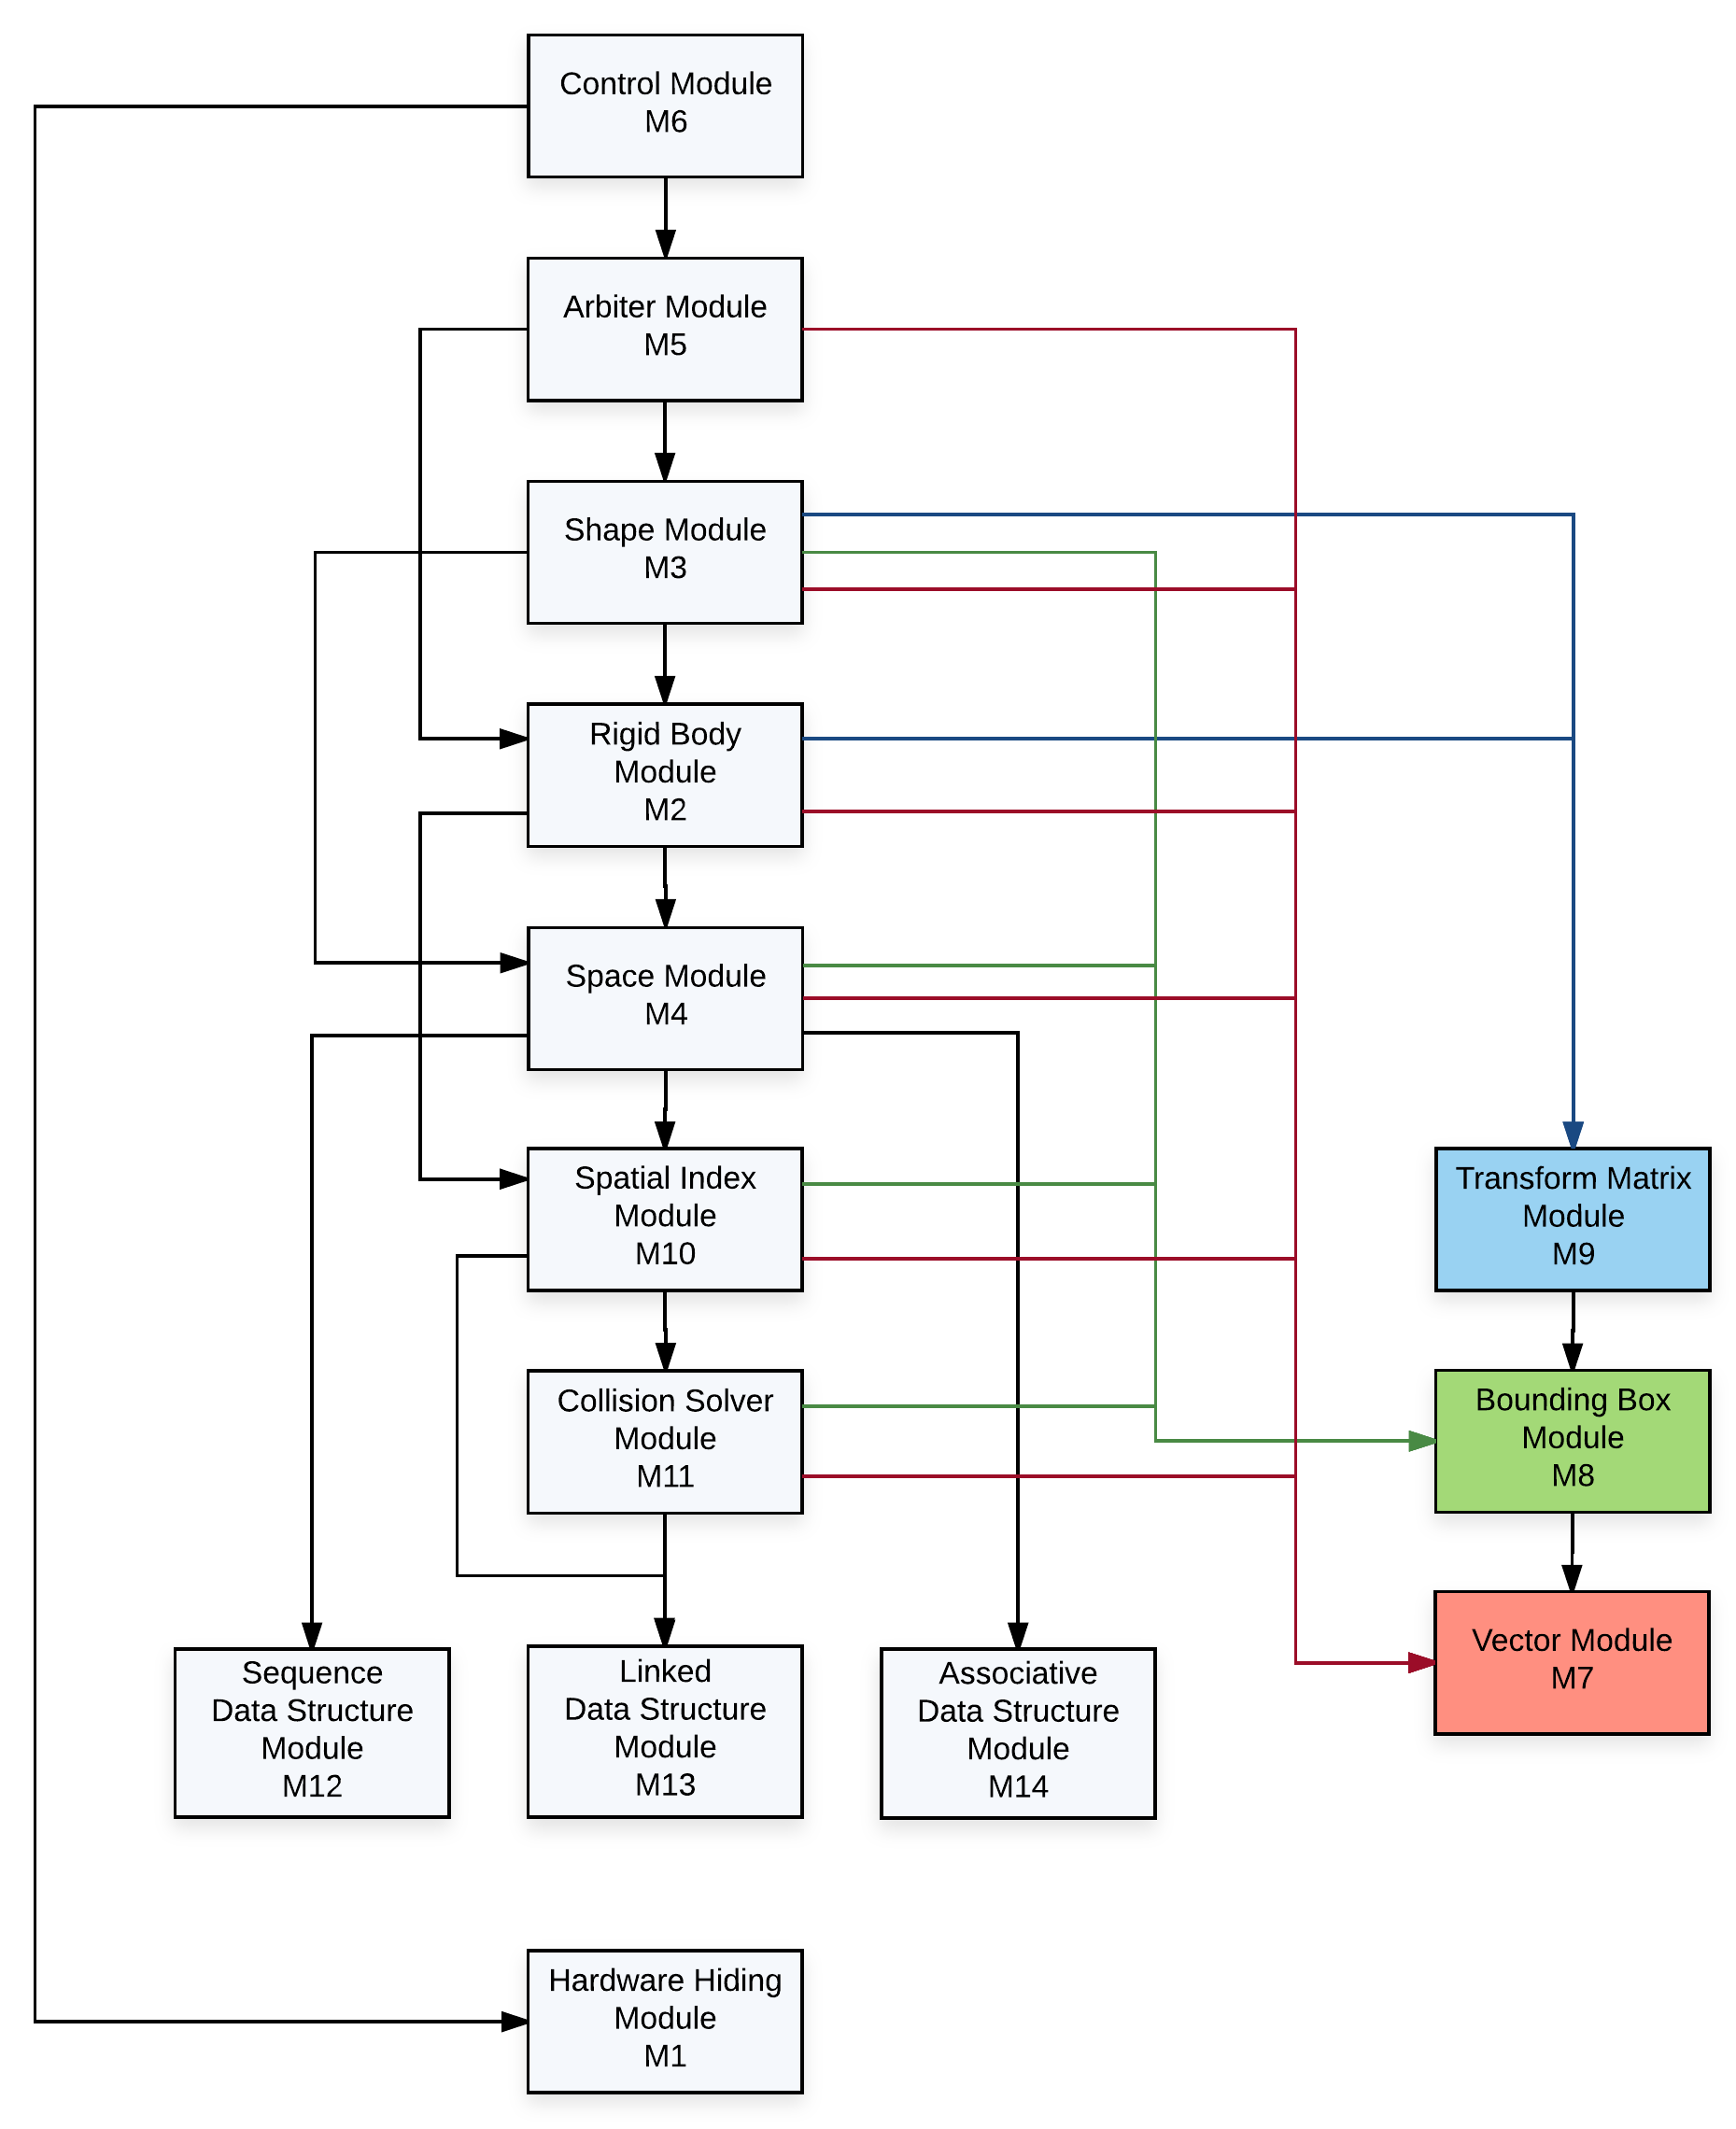
\includegraphics[width=0.71\textwidth]{uses}
}
\caption{\label{Fig_uses}Use hierarchy among Modules}
\end{center}
\end{figure}

\section{Inheritance Hierarchy Between Modules} \label{SecInheritance}
In this section the inheritance hierarchy between modules is provided (Figure \ref{Fig_Inheritance}).
Modules in the lower level of the hierarchy inherit properties from the higher levels.
\begin{figure}[htbp]
\begin{center}
%\rotatebox{-90}
{
 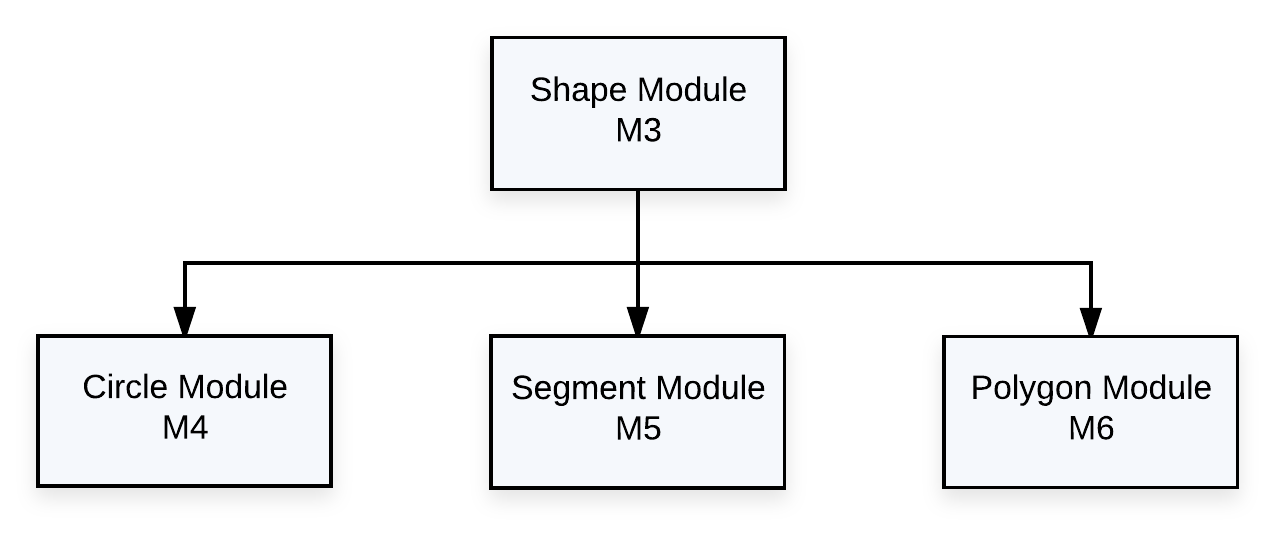
\includegraphics[width=0.75\textwidth]{inherit.png}
}
\caption{\label{Fig_Inheritance}Inheritance hierarchy among Modules}
\end{center}
\end{figure}

\bibliographystyle {plainnat}
\bibliography {../Physics_Game_Library}

\end{document}